\chapter{Background}
\label{ch:background}
%%%%%%%%%%%%%%%%%%%
% - description of foundational knowledge required to understand the thesis
%%%%%%%%%%%%%%%%%%%

This chapter explains the fundamental topics required to understand this thesis.

\section{Semantic Web Topics}
The following topics come from the research area of Semantic Web.
Since this thesis focuses mostly on the implementation and deployment of the Basilisk platform, these topics are mostly introduced to give a basic understanding of the context in which the Basilisk platform is used.

\subsection{Knowledge Graphs} 
\label{sec:knowledge_graphs}
Knowledge Graphs are graphs intended to represent knowledge of the real world or smaller scenarios.
The knowledge stored in Knowledge Graphs is modeled in a graph-based structure. 
Nodes represent entities which are connected by various types of relations, represented by labeled edges in the graph.
This has the benefit to represent complex relations between different nodes and edges\cite{hoganKnowledgeGraphs2021}.

The simplest knowledge graph consists of three elements.
The subject entity, the object entity and the labeled edge between them describing their relation.
This atomic data entity is called triple.
In figure \ref{fig:example-knowledge-graph} a simple example of a knowledge graph is shown.

\begin{figure}[tbph]
	\centering
	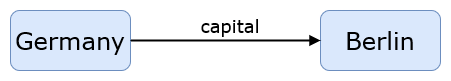
\includegraphics[width=0.4\textwidth]{figures/knowledge-graph-diagram}
	\caption{Simple Knowledge Graph}
	\label{fig:example-knowledge-graph}
\end{figure}

Since a graph structure is hard to store in a classic relational database a different type of storage is needed.
The special kind of database developed to store knowledge graphs are called \tsp{}.


\subsection{RDF}
\label{sec:rdf}
The Resource Description Framework is a framework for describing data and knowledge in a standardized way \cite{RDFConceptsAbstract} and it is part of the W3C standard.
The information is written down as subject-predicate-object triples, representing the basic structure that is also present in Knowledge Graphs (\ref{sec:knowledge_graphs}).
The elements of those triples can be IRIs (internationalized resource identifiers), blank nodes or datatyped literals.

RDF graphs can be encoded with different syntax styles.
A popular syntax is TURTLE \cite{RDFTurtle} which is a compact way of writing down a RDF graph structure.
Using the example of section \ref{sec:knowledge_graphs}, the knowledge graph would be represented with the TURTLE syntax seen in figure \ref{fig:rdf_turtle}.
The first two lines of the TURTLE document define abbreviations for the used IRIs so that the triple in line three is more readable.

\begin{figure}[tbph]
	\begin{lstlisting}
@prefix dbr: <http://dbpedia.org/resource/> .
@prefix dbo: <http://dbpedia.org/ontology/> .
dbr:Germany dbo:capital dbr:Berlin .
	\end{lstlisting}
	\caption{Example of an RDF graph in TURTLE syntax.}
	\label{fig:rdf_turtle}
\end{figure}


\subsection{\ts{}}
\label{sec:triplestores}
\tsp{} are a special kind of database developed to easily store and access knowledge graphs through queries.
Example of \tsp{} are Tentris\cite{bigerlTentrisTensorBasedTriple2020}, GraphDB\footnote{\url{https://graphdb.ontotext.com/}}, Virtuoso\footnote{\url{https://virtuoso.openlinksw.com/}}, or Jena TDB\footnote{\url{https://jena.apache.org/documentation/tdb/}}.

This thesis focuses on \tsp{} that accept SPARQL queries, since the used benchmark framework \iguana{} is using the SPARQL endpoint to perform benchmarks (see section \ref{sec:iguana}).


\subsection{SPARQL}
\label{sec:sparql}
SPARQL (SPARQL Protocol and RDF Query Language)\cite{harrisSPARQLQueryLanguage} is a query language for manipulating and retrieving RDF data stored in \tsp{}.
Just like RDF, SPARQL is part of the W3C recommendations for technologies in the semantic web.

The syntax for SPARQL queries looks similar to the SQL syntax, since its main parts are also a \texttt{SELECT} clause stating which variables to query for, following by an \texttt{WHERE} clause giving restrictions.

Queries can contain optional graph patterns, conjunctions, disjunctions, as well as aggregation functions.
These extension can help formulate more complex queries.

Following the example from section \ref{sec:knowledge_graphs} and \ref{sec:rdf} there are two example SPARQL queries in figure \ref{fig:sparql_example}.
Executed against the DBPedia SPARQL endpoint\footnote{\url{https://dbpedia.org/sparql}} the following results can be found:

The first example query requests the variable which matches the \texttt{WHERE} clause searching for the capital of Germany, which is \texttt{dbr:Berlin}.
The second query requests all relationships that can be found between Germany and Berlin, which will return \texttt{dbo:capital}, which we expected, but also \texttt{dbo:wikiPageLink}, which means that there is a link from the Wikipage of Germany to the Wikipage of Berlin.

\begin{figure}[tbph]
	\begin{lstlisting}
PREFIX dbr: <http://dbpedia.org/resource/>
PREFIX dbo: <http://dbpedia.org/ontology/>

SELECT ?capital
WHERE {
	dbr:Germany dbo:capital ?capital .
}

---

SELECT ?relation
WHERE {
	dbr:Germany ?relation dbr:Berlin .
}
	\end{lstlisting}
	\caption{SPARQL query examples}
	\label{fig:sparql_example}
\end{figure}


\section{Software Development}
The following topics can be grouped under the field of software development.
For the topic of benchmarks (section \ref{sec:benchmark}) we focus on database benchmarks and especially \ts{} benchmarks, since this is the main goal of the Basilisk platform.
The sections Microservice and Microservice Architecture (\ref{sec:microservice}, \ref{sec:microservice_architecture}) explain the basic idea and concept of the microservice architecture style.
In the sections RabbitMQ and Spring (\ref{sec:rabbitmq}, \ref{sec:spring}) we give a short introduction and description of the main technologies that are used for the development of the Basilisk platform.

\subsection{Benchmark}
\label{sec:benchmark}
Benchmarks for databases consist of a data set and a set of operations or queries which will be performed on the data set.
These operations are designed to simulate a particular type of workload to the system.
The goal of a benchmark is to measure different metrics for a better comparison between various systems.
Metrics used for databases and \tsp{} are \eg, number of executed queries and queries per second\cite{IguanaDocumentationMetrics}.

A distinction is made between micro and macro benchmarks.
Micro benchmarks focus on testing the performance of single components of a system.
Macro benchmarks test the performance of a system as a whole.
The benchmarks performed by the Basilisk platform, which will be set up in this thesis, will only perform macro benchmarks.

\subsection{Microservice}
\label{sec:microservice}
A microservice is an independently deployable piece of software that only implements functionalities that are closely related to the main task of the service \cite{dragoniMicroservicesYesterdayToday2017}.
The microservice interacts via messages through a defined protocol with other services.

\subsection{Microservice Architecture}
\label{sec:microservice_architecture}
A microservice architecture is a way of designing a software application as a set of microservices which interact with each other to provide the designed functionality \cite{dragoniMicroservicesYesterdayToday2017, MicroservicesHttpsMartinfowler}.
The functionality of the application gets split up into microservices which interact only through a defined protocol of messages.
This allows for a distributed system in which the individual service could be implemented in different programming languages and also could be located on different servers.
Microservices can be individually deployed and managed.


\subsection{RabbitMQ}
\label{sec:rabbitmq}
RabbitMQ is an open-source message broker that supports different messaging protocols like MQTT, STOMP and AMQP.
The system supports a variety of asynchronous messaging techniques \eg, delivery acknowledgment, flexible routing\cite{RabbitMQWebsiteHttps}.

In the context of the Basilisk platform we only need the most basic functionalities of message queues with a single producer and a single consumer.
Since RabbitMQ is a widely used message broker, the Spring framework (\ref{sec:spring}) already comes with the needed libraries to work with the RabbitMQ system.


\subsection{Spring and Spring Boot}
\label{sec:spring}
Spring is a widespread Java framework which supports the development process for various kinds of java applications and systems.
\todo{fill}





















